% TLCD 1.0 manuscript for Scientific Data
% English is used for the submitted manuscript. Chinese translations and
% author notes are retained as LaTeX comments beginning with "%".

\documentclass[pdflatex,sn-mathphys-num]{sn-jnl}

\usepackage{graphicx}
\graphicspath{{figures/}}
\usepackage{multirow}
\usepackage{amsmath,amssymb,amsfonts}
\usepackage{booktabs}
\usepackage{xcolor}
\usepackage{textcomp}
\usepackage{placeins}

\raggedbottom

\begin{document}
\newgeometry{margin=1in}

% TODO：按 Scientific Data 的最终标题要求重写；当前暂保留工作标题。
\title[TLCD 1.0]{TLCD 1.0: A Traffic Law Compliance Dataset for Autonomous Vehicles Based on Legal Driving-Behavior Monitoring}

\author[1]{\fnm{Chengxiang} \sur{Zhao}}\email{zhao\_cx25@mails.tsinghua.edu.cn}
% TODO: Add the complete author list, corresponding author and affiliations
% after confirmation by all contributors.
\affil*[1]{\orgdiv{School of Vehicle and Mobility}, \orgname{Tsinghua University}, \orgaddress{\city{Beijing}, \country{China}}}

% 摘要：待 Methods、Data Records 和 Technical Validation 定稿后再写，避免提前锁定错误叙事。
\abstract{[To be completed after the Methods, Data Records and Technical Validation sections have been finalized.]}

% 关键词：待全文术语统一后确定。
\keywords{traffic-law compliance, autonomous driving, real-world driving data, event-level dataset}

\maketitle

\section{Background \& Summary}\label{sec:background-summary}

% TODO：本节待 Methods 定稿后编写。建议简要包括：
% 1. 交通法规合规性在自动驾驶评估中的意义；
% 2. 现有数据集在法规条款、合规标签和可追溯证据方面的空缺；
% 3. TLCD 1.0 的数据规模、主要构成与复用价值；
% 4. 数据的地理、法规版本和车辆平台边界。
[To be drafted after completion of the Methods section.]

\section{Methods}\label{sec:methods}

% 本节介绍 TLCD 1.0 的数据采集平台、道路采集、在线合规性监测、事件触发式记录以及离线数据处理流程。
This section describes the data acquisition platform, road-data collection, online compliance monitoring, event-triggered recording and offline data-processing procedures used to construct TLCD 1.0.

\subsection{Data acquisition platform}\label{subsec:data-acquisition-platform}

% TLCD 1.0 使用一辆配备 L3 级自动驾驶系统的一汽红旗 EH7 研发样车采集（图 1）。车载感知与定位系统包括 7 个摄像头、3 个激光雷达、5 个毫米波雷达、全球导航卫星系统/惯性导航系统（GNSS/INS）以及高精地图。车载系统融合这些输入，输出自车状态、最多 30 个周边目标的融合信息，以及车道级地图信息。TLCD 1.0 公开覆盖 6 个观测方向的 7 路原始摄像头视频，包括 30° 长焦和 120° 广角两路前视视频、1 路后视视频和 4 路侧向视频，同时提供相应的自车、目标和地图结构化数据。数据集不包含原始激光雷达、毫米波雷达和 GNSS/INS 测量。
The data acquisition platform was built on a FAW Hongqi EH7 engineering prototype equipped with an L3 autonomous driving system, as shown in Fig.~\ref{fig:data-acquisition-platform}. The vehicle integrates a multi-source perception and localization suite, including seven cameras, three LiDARs, five millimeter-wave radars, a GNSS/INS fused positioning system, high-definition maps, and an onboard computing module. The cameras, LiDARs, and radars provide complementary information for object detection, classification, tracking, and dynamic environment perception, while the GNSS/INS and HD map modules provide high-precision vehicle pose, road topology, and lane-level semantic information.  

\begin{figure}[htbp]
\centering
\includegraphics[width=0.9\textwidth]{fig1.png}
% 一汽红旗 EH7 研发样车及其车载感知系统。
\caption{FAW Hongqi EH7 engineering prototype and its onboard sensing suite.}
\label{fig:data-acquisition-platform}
\end{figure}

\begin{figure}[htbp]
\centering
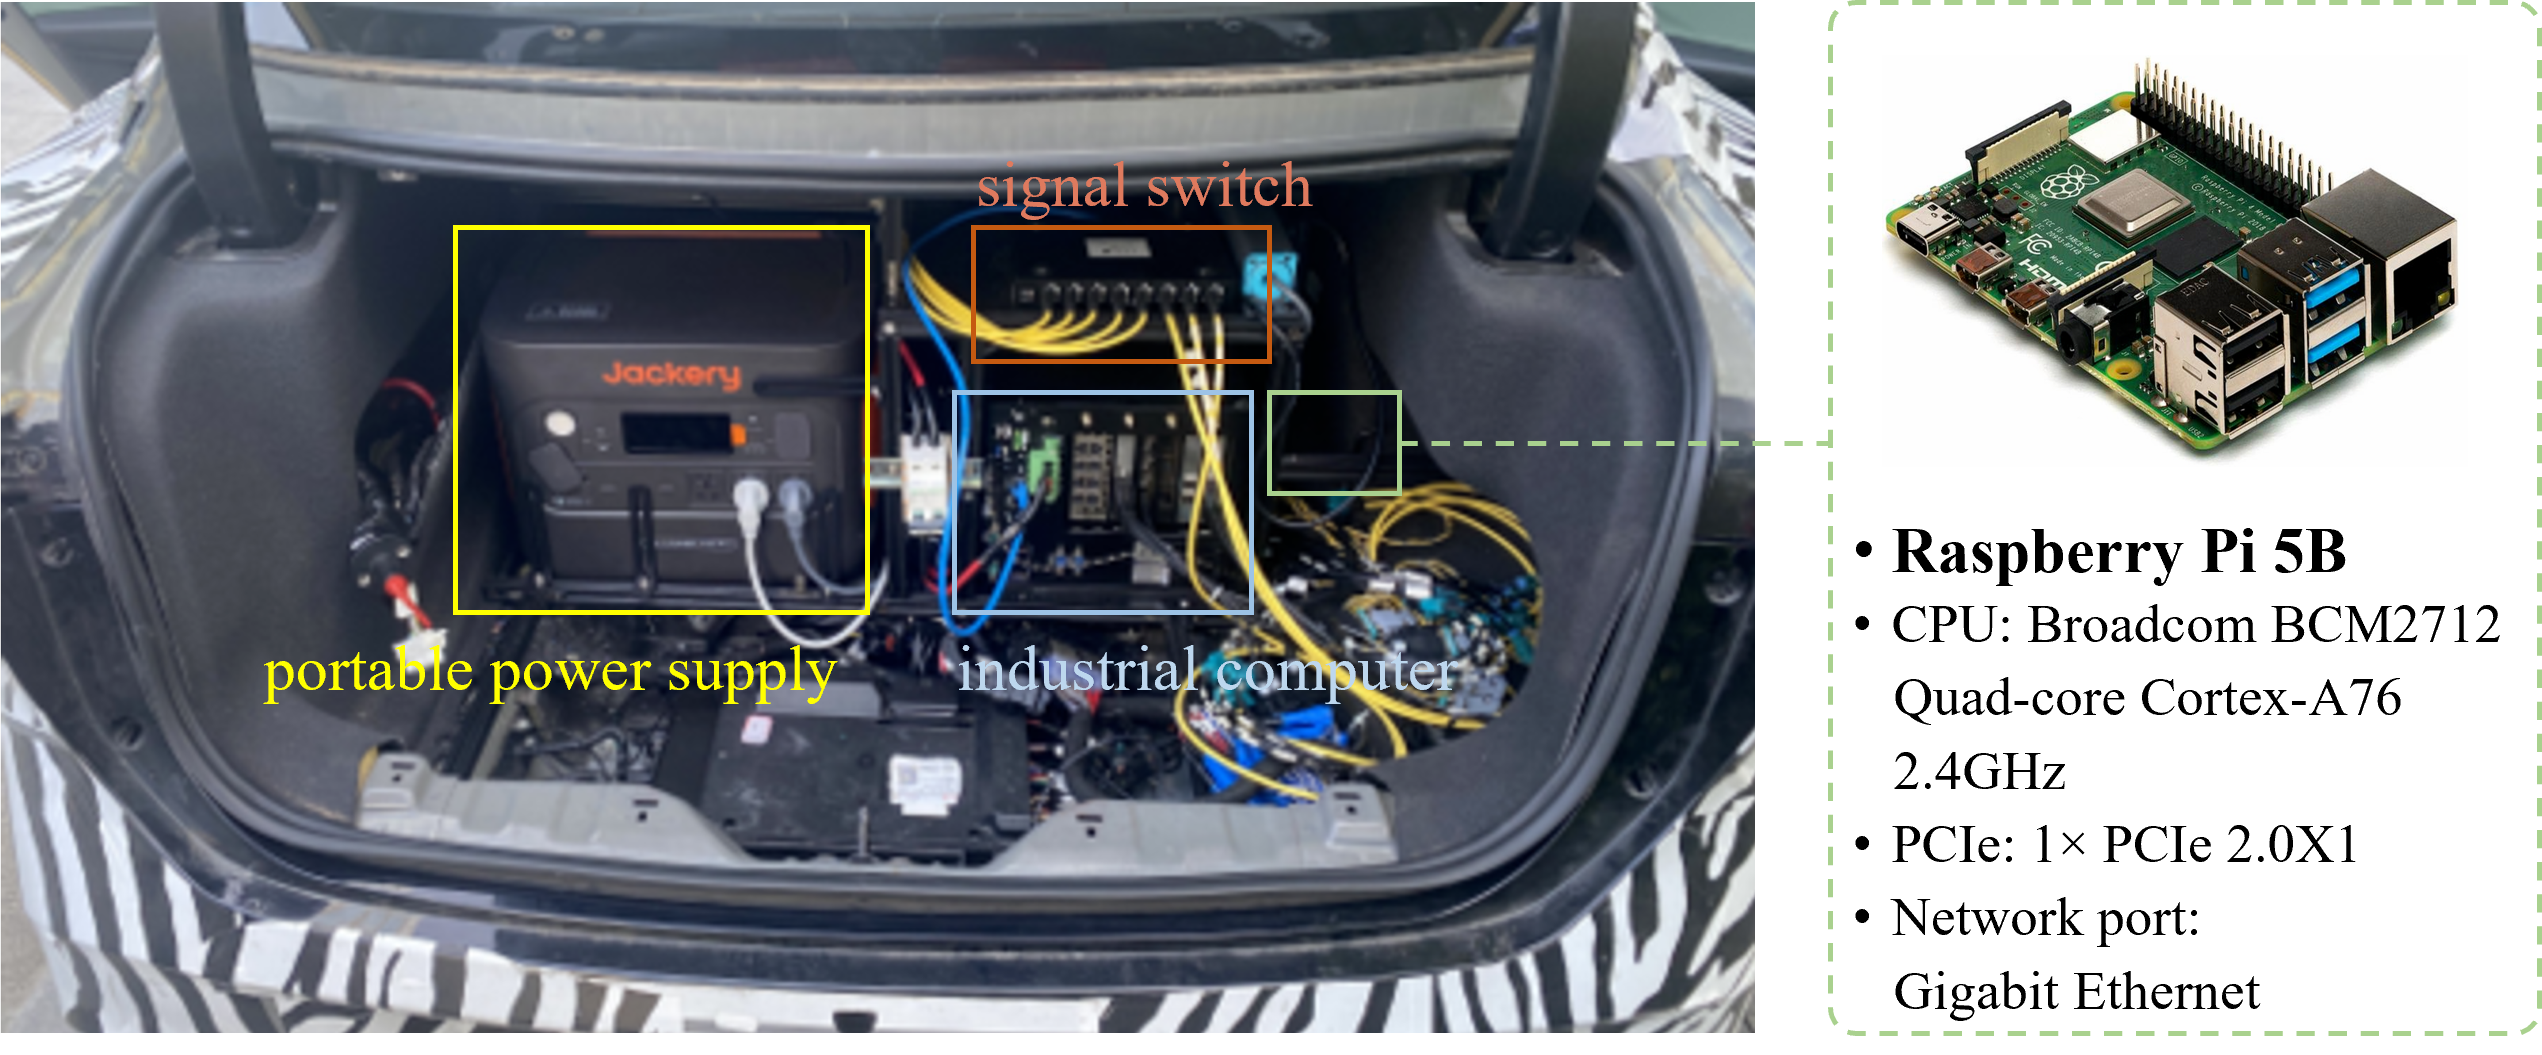
\includegraphics[width=0.9\textwidth]{fig2.png}
% 安装在车辆后备箱内的外部交通法规合规性监测与事件触发式数据记录系统。
\caption{External traffic-law-compliance monitoring and event-triggered data-recording system installed in the rear compartment.}
\label{fig:external-monitoring-setup}
\end{figure}

% 车辆后备箱内安装了一套外部监测和事件触发式记录系统（图 2），由运行 Ubuntu 20.04 的工业计算机、以太网交换机、树莓派和独立电源组成。交通法规合规性监测算法被部署在树莓派中，作为独立的边缘计算单元运行。工业计算机运行车端系统的可视化和数据采集软件，以及用于提取交通法规合规性监测所需信号的中间件。这些信号使用 Protocol Buffers 序列化，并通过以太网以 UDP 方式发送至树莓派。树莓派以 100 Hz 频率执行合规性监测，并通过同一通信接口返回包含事件触发信号在内的监测结果。数据采集软件收到事件触发信号后，保存该信号所指定时间区间内的车辆数据，而不是连续记录整个行程。工业计算机和树莓派均与车端时钟同步。
An external monitoring and event-triggered recording system was installed in the rear compartment of the vehicle (Fig.~\ref{fig:external-monitoring-setup}). It comprised an industrial computer running Ubuntu 20.04, an Ethernet switch, a Raspberry Pi, and an independent power supply. The traffic-law-compliance monitoring algorithm was deployed on the Raspberry Pi as an independent edge-computing unit.
The industrial computer ran the vehicle-system visualization and data-acquisition software, together with middleware that extracted the signals required by the traffic-law-compliance monitoring algorithm. These signals were serialized using Protocol Buffers and transmitted to the Raspberry Pi over Ethernet using the User Datagram Protocol (UDP). The Raspberry Pi performed compliance monitoring at 100 Hz and returned the monitoring outputs, including event-trigger signals, through the same communication interface. Upon receiving an event-trigger signal, the data-acquisition software retained the vehicle data corresponding to the specified time interval rather than recording the entire trip continuously. The industrial computer and Raspberry Pi were synchronized with the vehicle-side clock.



\subsection{Road-data collection}\label{subsec:road-data-collection}

% 连续道路测试数据采集于南京和长春的高速公路及城市快速路实际交通环境。用于数据集构建的长春和南京道路测试记录分别覆盖 2024 年 8 月 27 日至 10 月 22 日和 2024 年 9 月 10 日至 10 月 23 日。测试主体路线为预先选定，个别测试过程中也会临时调整路线。人工驾驶数据既包括独立的人工驾驶测试，也包括驾驶员接管后的路段；两种驾驶模式按测试计划切换。
Continuous road-test data were collected under real-world traffic conditions on highways and urban expressways in Nanjing and Changchun, China. The road-test records retained for dataset construction span 27 August to 22 October 2024 in Changchun and 10 September to 23 October 2024 in Nanjing. Most routes were selected in advance, with temporary route adjustments made during individual tests. The manual-driving data comprise both dedicated manual-driving tests and road sections following driver takeover; transitions between manual and automated driving followed the test plan.

% 表 1 汇总了用于构建 TLCD 1.0 的全部连续道路测试的里程和时长。这些统计数据表征的是事件触发时间段所源自的道路测试规模，而非公开事件窗口的时长之和。按当前统计，道路测试总里程为 2034.94 km，总时长为 35.18 h，其中人工驾驶和自动驾驶里程分别为 1132.80 km 和 902.14 km。图 3 在卫星影像上显示了有效行驶轨迹在两座城市的空间覆盖，红点表示轨迹可视化使用的局部坐标原点。
Table~\ref{tab:driving-mileage} summarizes the mileage and duration of all continuous road tests used to construct TLCD 1.0. These statistics characterize the road tests from which event-triggered intervals were retained, rather than the summed duration of the released event windows. Based on the current statistics, the road tests covered 2,034.94~km and 35.18~h, comprising 1,132.80~km in manual driving mode and 902.14~km in automated driving mode. Figure~\ref{fig:collection-routes} shows the spatial coverage of the valid driving trajectories in the two cities over satellite imagery. The red point marks the local coordinate origin used for trajectory visualization.

% TODO：表 1 中的里程和时长为当前临时统计值，待重新统计后更新正文及表格。

\begin{table}[htbp]
\centering
\caption{Driving mileage and duration of TLCD 1.0}\label{tab:driving-mileage}%
\begin{tabular}{@{}ccccccc@{}}
\toprule
\multirow{2}{*}{Collection site} & \multicolumn{3}{@{}c}{Mileage (km)} & \multicolumn{3}{@{}c@{}}{Duration (h)} \\
\cmidrule(lr){2-4}\cmidrule(l){5-7}
& Human-driving & Autonomous-driving & Total & Human-driving & Autonomous-driving & Total \\
\midrule
Nanjing & 1081.79 & 268.35 & 1350.14 & 9.26 & 16.21 & 25.47 \\
Changchun & 51.01 & 633.79 & 684.80 & 1.73 & 7.98 & 9.70 \\
\midrule
Total & 1132.80 & 902.14 & 2034.94 & 10.99 & 24.19 & 35.18 \\
\botrule
\end{tabular}
\end{table}

\begin{figure*}[htbp]
\centering
\includegraphics[width=0.95\textwidth]{fig3.png}
% 南京和长春的有效行驶轨迹空间分布。
\caption{Spatial distribution of valid driving trajectories in Nanjing and Changchun.}
\label{fig:collection-routes}
\end{figure*}

\subsection{Online compliance monitoring and event-triggered recording}\label{subsec:event-recording}

% 本数据集所监测的法规条款选自《中华人民共和国道路交通安全法实施条例》中高速公路驾驶场景下的常见要求，并归纳为最高限速、最低限速、跟车距离、横向距离、变道、连续变道、道路标线合规和超车八类事件。
The monitored provisions were selected from commonly encountered requirements for expressway driving in the \textit{Regulation on the Implementation of the Road Traffic Safety Law of the People's Republic of China} \cite{statecouncil2017regulation}. They were organized into eight event categories: maximum-speed limit, minimum-speed limit, following distance, lateral distance, lane change, continuous lane change, road-marking compliance, and overtaking.

% 自然语言法规向机器可执行的触发条件、阈值和逻辑判断的转换沿用前期工作。该工作构建了基于触发机制的分层在线合规性监测系统，其结构如图4上部所示。每项法规均采用“触发条件—逻辑判断”结构表示：触发条件用于判断当前道路环境和驾驶行为是否属于法规的适用场景，满足触发条件后，逻辑判断给出相应的合规结果。系统综合考虑不同法规之间的共用触发条件、触发优先级和隐含触发前提，并通过分层触发架构组织监测逻辑，从而减少对共用前提的重复判断并支持实时监测。实车运行期间，在线监测算法持续接收自车状态、感知信息和地图信息等多源车载输入，并以100 Hz的固定频率输出各项法规的触发状态、合规状态和关键中间变量。
The conversion of natural-language provisions into machine-executable trigger conditions, thresholds, and logical judgements followed our previous work \cite{yu2024online}. In that work, we developed a trigger-based hierarchical online compliance-monitoring system, as illustrated in the upper part of Fig.~\ref{fig:framework}. Each traffic regulation was represented using a \textit{trigger-condition--logical-judgement} structure. The trigger condition determined whether the current road environment and driving behaviour fell within the scope of a specific regulation. Once triggered, the logical judgement evaluated compliance with that regulation. The system accounted for shared trigger conditions, trigger priorities, and implicit triggering prerequisites across regulations, and organized the monitoring logic within a hierarchical trigger architecture. This organization reduced repeated evaluation of common prerequisites and supported real-time monitoring. During on-road operation, the algorithm continuously received multi-source onboard inputs, including ego-vehicle states, perception information, and map information, and produced the trigger state, compliance state, and key intermediate variables for each regulation at a fixed rate of 100~Hz.

% 连续逐帧结果被转换为标准化事件反馈信号Ei，其中RT为法规事件类别，FT为反馈特征类型，ks和ke为同步时间轴上的事件起止位置，tb为类别相关的前后缓冲配置。该信号定义了工控机需要保存的精确时间窗口。
The continuous frame-level outputs were converted into a standardized event-feedback signal
\begin{equation}
E_i = \{R_T, F_T, k_s, k_e, t_b\},
\label{eq:event-feedback}
\end{equation}
where $R_T$ denotes the regulation-event category, $F_T$ identifies the event-defining feedback feature, $k_s$ and $k_e$ are the start and end positions on the synchronized timeline, and $t_b$ specifies the category-dependent pre- and post-event buffers. Thus, $E_i$ defines the exact temporal window that must be retrieved by the recording computer rather than merely issuing a binary recording command.

\begin{figure*}[htbp]
\centering
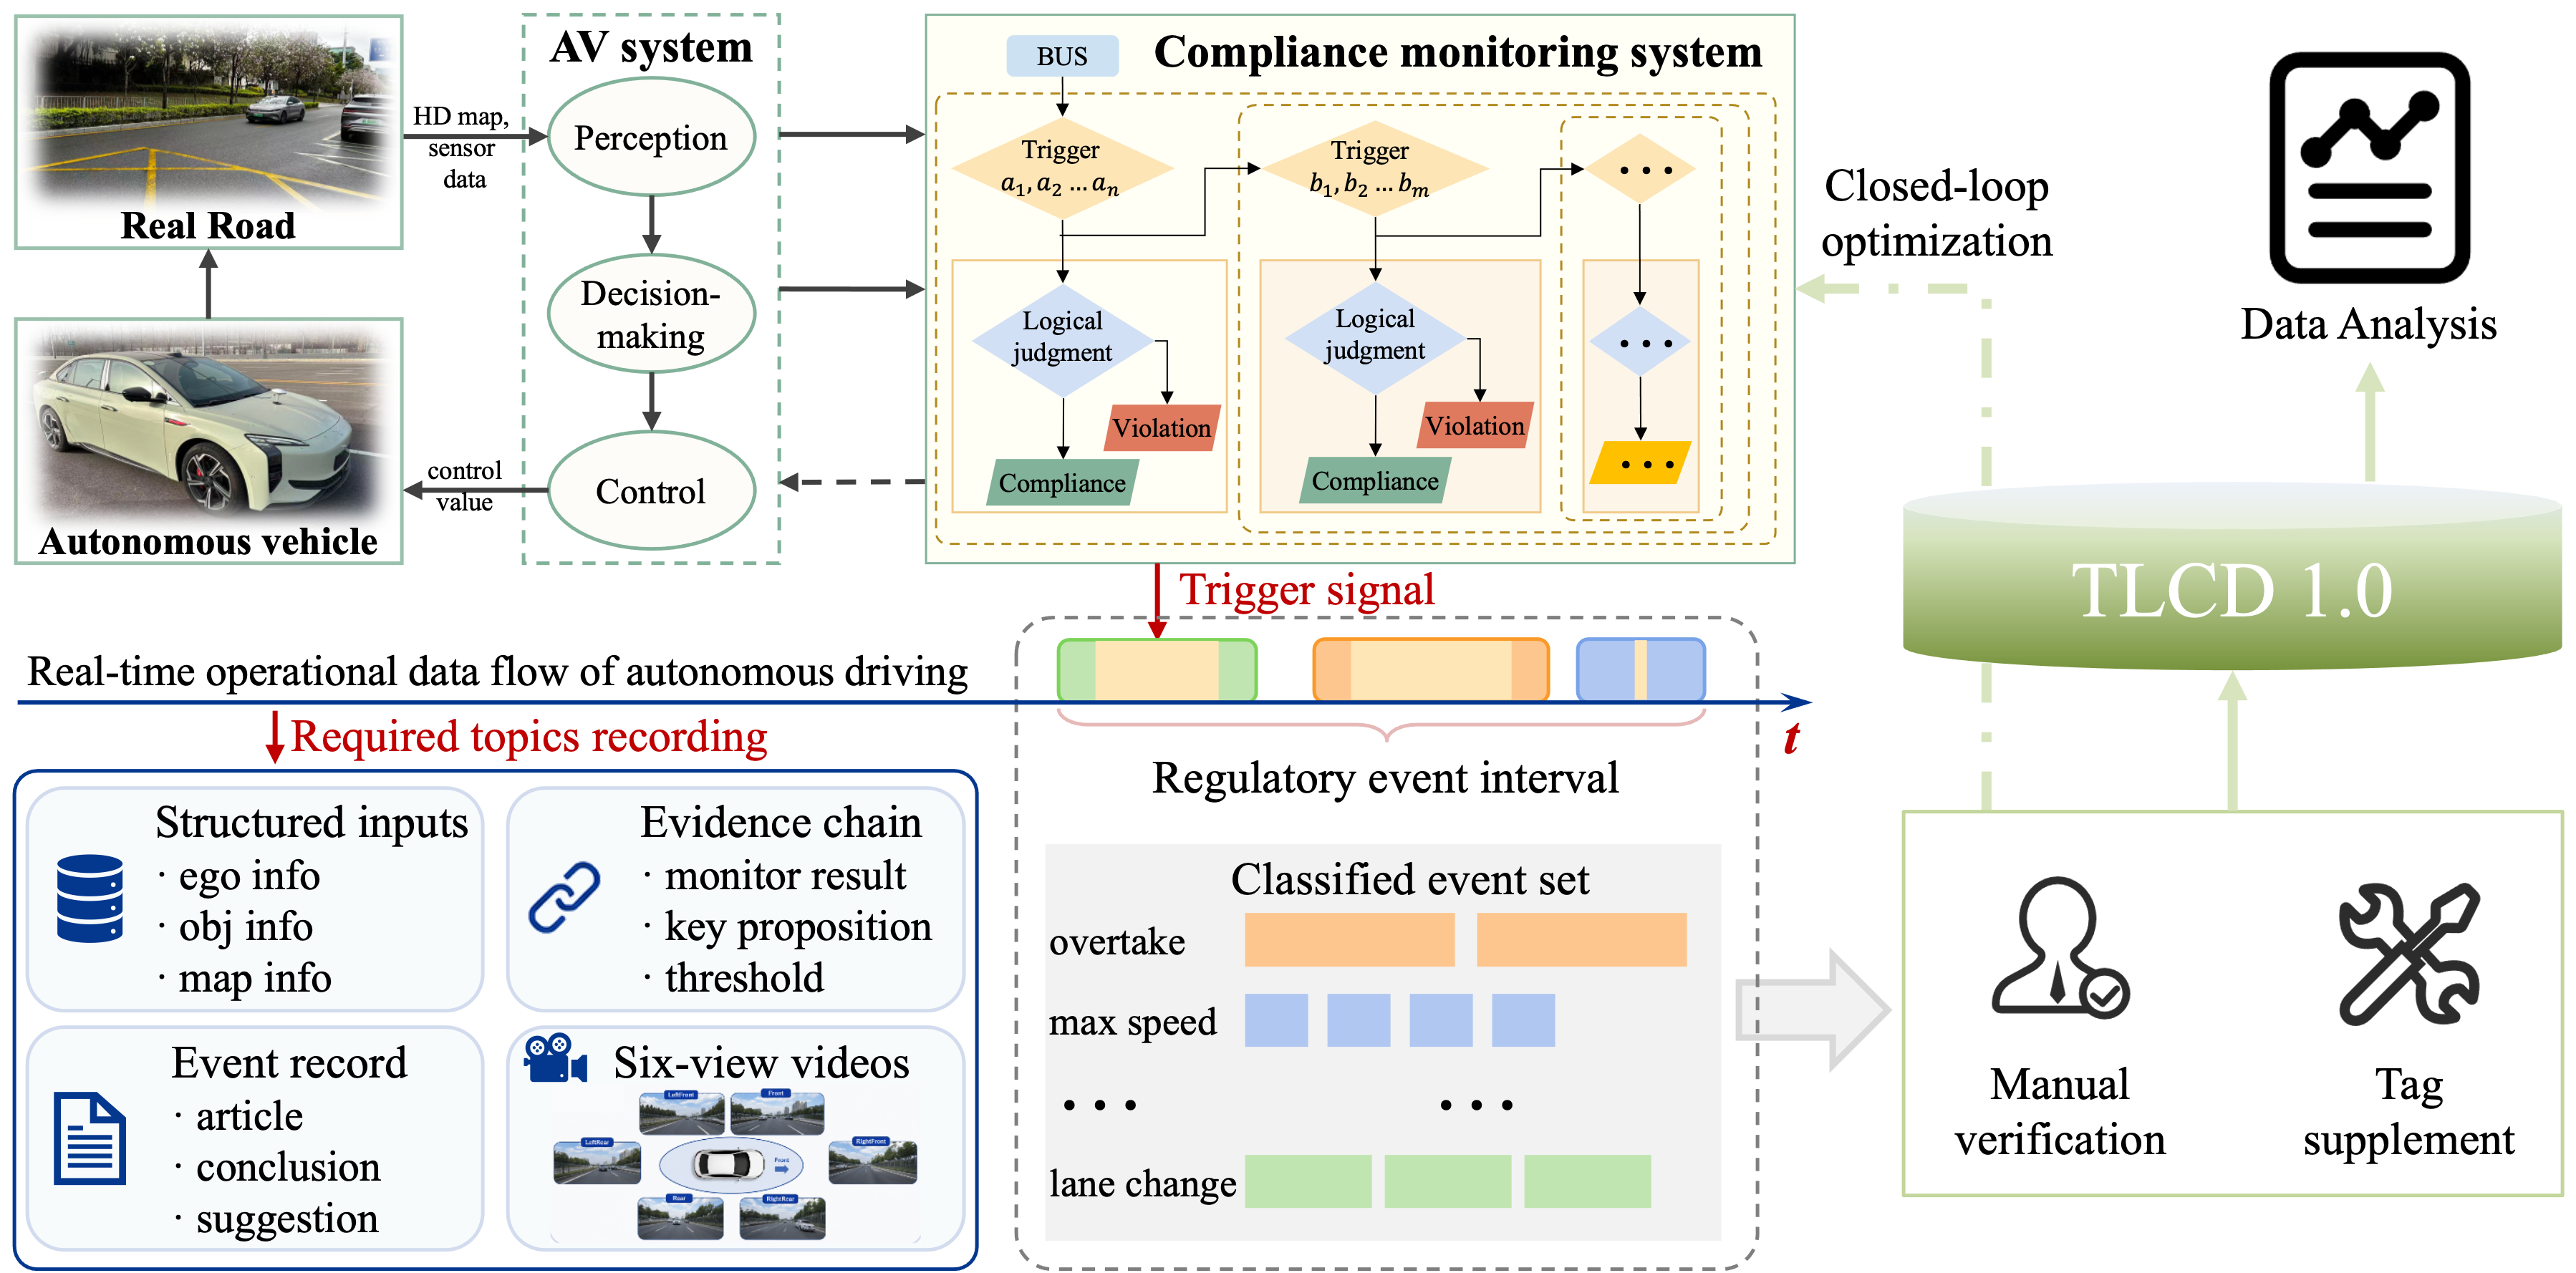
\includegraphics[width=0.96\textwidth]{fig4.png}
\caption{Online compliance monitoring and event-triggered recording workflow. The hierarchical monitor produces frame-level trigger and compliance states; category-specific event feedback defines the temporal window; and the IPC retrieves synchronized topics from rolling buffers. Final event-level labels are assigned during offline processing.}
\label{fig:framework}
\end{figure*}

% 本次事件分割策略依据各类法规相关事件的语义特征制定。针对限速、跟车距离要求等长时间连续状态约束类事件，以触发状态切换时刻或违规结果产生时刻为基准确定事件窗口；针对横向距离关联事件、道路标线关联事件等过程型驾驶行为，将有效触发区间的起止时间作为事件基准点；针对变道、超车等存在驾驶状态转换的行为，以完整状态转换区间的起止时间划定事件窗口。为保留上下文关联信息，通常在区间两侧各保留3秒的上下文数据（$t_b$），覆盖触发前的车辆行驶状态、与周边交通参与者的交互过程以及触发结束后的行为恢复过程。此外，为抑制短暂信号波动造成的片段碎片化问题，对大多数类别时长小于1秒的无效间断区间做了填补处理。表中给出了各类事件窗构造的原则。
The event-segmentation strategy was defined according to the temporal semantics of the eight event categories. For long-duration continuous-state constraints, including speed-limit and following-distance requirements, event windows were anchored at a transition in the trigger state or the onset of a violation. For process-based events related to lateral distance or road markings, the onset and termination of the effective trigger interval served as the event reference points. For behaviours involving a driving-state transition, including lane changes and overtaking, the event window spanned the complete transition interval. To preserve contextual information, 3~s of data were generally retained on each side of the interval ($t_b$), covering the pre-trigger driving state, interactions with surrounding traffic participants, and behavioural recovery after the trigger ended. In addition, inactive gaps shorter than 1~s were bridged for most event categories to reduce fragmentation caused by transient signal fluctuations. Table~\ref{tab:event-window-parameters} summarizes the category-specific rules used to construct the event windows.

% 最高限速：1是以触发状态切换时刻作为锚点；2是2-6s短时违规，保留整个区间作为锚点区间；3是超过6s的长时违规，以合规状态切换时刻作为锚点。
% 最低限速：时间窗口锚定在合规的限速标志状态切换时刻，或是高速公路上连续6s无标志的稳定区间。
% 跟车距离：有效触发区间大于2秒的片段予以保留，时长不超过6秒的区间完整留存；超过6秒的区间仅围绕合规状态变更点进行截取。
% 横向距离：有效触发区间大于1秒的片段予以保留，时长不超过6秒的区间完整留存；超过6秒的区间仅围绕合规状态变更点进行截取。
% 变道：保留持续压线时长大于 2 秒且小于 16 秒的潜在完整变道触发行为。
% 连续变道：当两次有效变道触发的压线时间间隔小于 10 秒时，将其配对为连续变道行为，保留完整的连续变道过程。
% 压线：有效触发区间大于0.5秒的片段予以保留；所有违规区间均予以保留。为减少数据冗余，每5min内，0.5–2 秒和 2–6 秒这两个有效时长区间内最多保留两个合规样本。
% 超车：当两次有效变道触发的压线方向相反且压线时间间隔小于 20 秒时，将其配对为超车行为，保留完整的超车过程。

\begin{table*}[htbp]
\caption{Temporal rules used for event-window construction.}
\label{tab:event-window-parameters}
\small
\begin{tabular}{@{}p{0.19\textwidth}p{0.76\textwidth}@{}}
\toprule
Event category & Event-window construction rule \\
\midrule
Maximum-speed limit & Event windows were anchored in one of three ways: at a trigger-state transition; across the complete interval for short violations lasting 2--6~s; or at a compliance-state transition for long violations lasting more than 6~s. \\
Minimum-speed limit & Event windows were anchored at valid transitions in the detected speed-limit-sign state or at contiguous, stable 6-s intervals without a speed-limit sign on expressways. \\
Following distance & Effective trigger intervals longer than 2~s were retained. Intervals of up to 6~s were preserved in full, whereas intervals longer than 6~s were extracted only around compliance-state transitions. \\
Lateral distance & Effective trigger intervals longer than 1~s were retained. Intervals of up to 6~s were preserved in full, whereas intervals longer than 6~s were extracted only around compliance-state transitions. \\
Lane change & Potential complete lane-change manoeuvres were retained when the lane-boundary-crossing trigger lasted more than 2~s and less than 16~s. \\
Continuous lane change & Two valid lane-change triggers were paired as a continuous lane-change event when their lane-boundary-crossing times were separated by less than 10~s. The complete paired process was retained. \\
Road marking & Effective trigger intervals longer than 0.5~s were retained, and all violating intervals were kept. To reduce redundancy, within each 5-min source segment, no more than two compliant samples were retained from each of the 0.5--2~s and 2--6~s duration ranges. \\
Overtaking & Two valid lane-change triggers with opposite lane-boundary-crossing directions were paired as an overtaking event when their crossing times were separated by less than 20~s. The complete paired process was retained. \\
\botrule
\end{tabular}
\end{table*}

% 树莓派将Ei通过车载以太网反馈给工控机。工控机持续维护滚动缓存，在接收到事件信号后，按照ks、ke和tb回取触发前数据并继续收集触发后数据，随后保存精确事件窗内的结构化主题、监测输出，以及覆盖六个观察方向的七路原始视频，因此无需连续保存整段道路测试数据。
The Raspberry Pi returned $E_i$ to the IPC through the same onboard Ethernet link used by the monitoring interface. The IPC maintained rolling buffers for the incoming streams. Upon receiving an event signal, it retrieved the required pre-trigger samples from the buffers, continued collecting data until the specified post-event boundary, and then stored the synchronized structured topics, monitoring outputs, and seven raw camera-video streams covering six viewing directions within the exact interval defined by $k_s$, $k_e$, and $t_b$. This design preserved the temporal context required for event interpretation without continuously recording the complete road test.

% 在线反馈仅用于识别并记录候选事件窗口。在线生成的逐帧合规状态与事件数据一同保存，但不直接作为公开数据集的最终事件级标签。最终标签根据事件窗口内的监测结果生成，并在离线人工复核中确认，必要时进行修正。完整流程见图4。
The online feedback was used only to identify and record candidate event windows. The frame-level compliance states generated online were stored with the corresponding event data but were not used directly as the final event-level labels released with the dataset. Instead, the final labels were derived from the monitoring results within each event window and then reviewed and, where necessary, corrected during offline manual verification. The complete workflow is illustrated in Fig.~\ref{fig:framework}.

\FloatBarrier

\subsection{Offline event processing and record generation}\label{subsec:offline-processing}

% 离线处理首先将已存储的车端数据流转换为标准化的事件级输入。程序选取自车状态、融合目标、地图和车道等所需主题，并将各信号映射到间隔为0.01 s的统一时间网格。对于每个目标时刻，保留时间戳不晚于该时刻的最近一条源数据，即采用零阶保持方式重采样至100 Hz。随后按照候选事件的起止位置裁剪数据窗口，并将时间转换为事件相对时间event_time。处理后的信号分别写入EgoInfo.csv、ObjInfo.csv和MapInfo.csv。
Offline processing first converted the stored vehicle-side data streams into standardized event-level inputs. The required ego-state, fused-object, map and lane topics were selected and mapped to a common time grid with a 0.01-s interval. At each target timestamp, the most recent source sample whose timestamp did not exceed the target was retained, corresponding to zero-order-hold resampling at 100~Hz. Each candidate event was then cropped using its start and end positions, and time was expressed relative to the event as \texttt{event\_time}. The processed signals were written to \texttt{EgoInfo.csv}, \texttt{ObjInfo.csv} and \texttt{MapInfo.csv}.

% 对每个事件类别，EvidenceChain.csv从上述三类结构化输入及在线监测过程中保存的类别相关变量中构建，其中包括判定阈值、触发状态和合规结果等关键证据。随后基于证据链生成record.json，以可读形式汇总事件元数据、适用法规、时间锚点、关键证据和合规判定。record.json不重复保存逐帧时序数据，因此法规判定仍可追溯至EvidenceChain.csv；对应视频也与同一事件窗口关联，用于后续复核和场景理解。
For each event category, \texttt{EvidenceChain.csv} was constructed from the three structured inputs and category-specific variables retained from online monitoring, including decision thresholds, trigger states and compliance results. A corresponding \texttt{record.json} file was then generated to summarize the event metadata, applicable regulation, temporal anchor, key evidence and compliance decision in a readable form. Because \texttt{record.json} does not duplicate the frame-level time series, each rule judgement remains traceable to \texttt{EvidenceChain.csv}. The associated videos were indexed to the same event window for subsequent review and scene interpretation.

% 所有候选事件均使用结构化事件文件、证据链和对应视频进行人工复核。可修复的数据问题在复核过程中予以修正，包括必要时修改Compliance_label；存在明显且无法可靠修复的上游数据问题的事件则被丢弃。仅结果可信的事件被纳入公开数据集。为进一步增强事件记录的可解释性并辅助质量检查，Qwen3.6-Plus被应用于全部八类事件。该模型结合EvidenceChain.csv中的结构化证据理解对应视频，生成场景描述和驾驶建议，并分别写入公开record.json中的Scenario_description_VLM和Driving_suggestion_VLM字段。在此过程中，模型还审视证据链与视频内容的一致性，将其认为证据链可能存在错误的事件标记为存疑事件，交由人工进行二次复核。模型生成的内容和判断不直接决定Compliance_label，最终结果仍由人工复核确定。
All candidate events underwent manual review using the structured event files, evidence chains and corresponding videos. Correctable data problems were repaired during review, including changes to \texttt{Compliance\_label} where necessary, whereas events with evident upstream-data defects that could not be reliably repaired were discarded. Only events whose results were considered reliable were included in the public dataset. To further improve the interpretability of the event records and support quality control, Qwen3.6-Plus was applied across all eight event categories. The model used the structured evidence in \texttt{EvidenceChain.csv} to interpret the corresponding videos and generate a scene description and driving suggestion, which were stored in the \texttt{Scenario\_description\_VLM} and \texttt{Driving\_suggestion\_VLM} fields of the public \texttt{record.json}, respectively. During this process, the model also examined the consistency between the evidence chain and the video content and flagged events for which it identified potential errors in the evidence chain as questionable cases for a second round of manual review. The model-generated content and assessments did not directly determine \texttt{Compliance\_label}; the final results remained subject to manual verification.

\section{Data Records}\label{sec:data-records}

% TODO：待数据仓库、DOI、版本和许可证确定后填写。
% 本节将简要说明数据库入口、城市/事件目录结构，以及 EgoInfo.csv、ObjInfo.csv、MapInfo.csv、EvidenceChain.csv、record.json 和 7 路视频的用途。详细法规映射与字段字典放在数据仓库的 DatasetInfo.md 中。
[Repository record, persistent identifier, version and concise file description to be added.]

\section{Data Overview}\label{sec:data-overview}

% TODO：本节按 Scientific Data 要求最终压缩为图 5、图 6 和一段中性的描述性文字。下列内容为现有工作稿。

% TLCD 1.0 共包含 5,173 个事件级记录，覆盖南京和长春两座城市、8 类交通法规事件以及 17 条适用法规（图 5）。南京和长春分别贡献 3,766 个（72.8\%）和 1,407 个（27.2\%）事件；自动驾驶和人工驾驶事件分别为 2,998 个（58.0\%）和 2,175 个（42.0\%）。全部数据中，3,455 个事件（66.8\%）标记为合规，1,718 个（33.2\%）标记为违规。
TLCD 1.0 contains 5,173 event-level records spanning eight traffic-law event categories and 17 applicable legal provisions across Nanjing and Changchun (Fig.~\ref{fig:event-statistics}). Nanjing and Changchun contributed 3,766 (72.8\%) and 1,407 (27.2\%) events, respectively. Automated and manual driving accounted for 2,998 (58.0\%) and 2,175 (42.0\%) events, respectively. Across the dataset, 3,455 events (66.8\%) were labelled compliant and 1,718 (33.2\%) were labelled as violations.

\begin{figure*}[htbp]
\centering
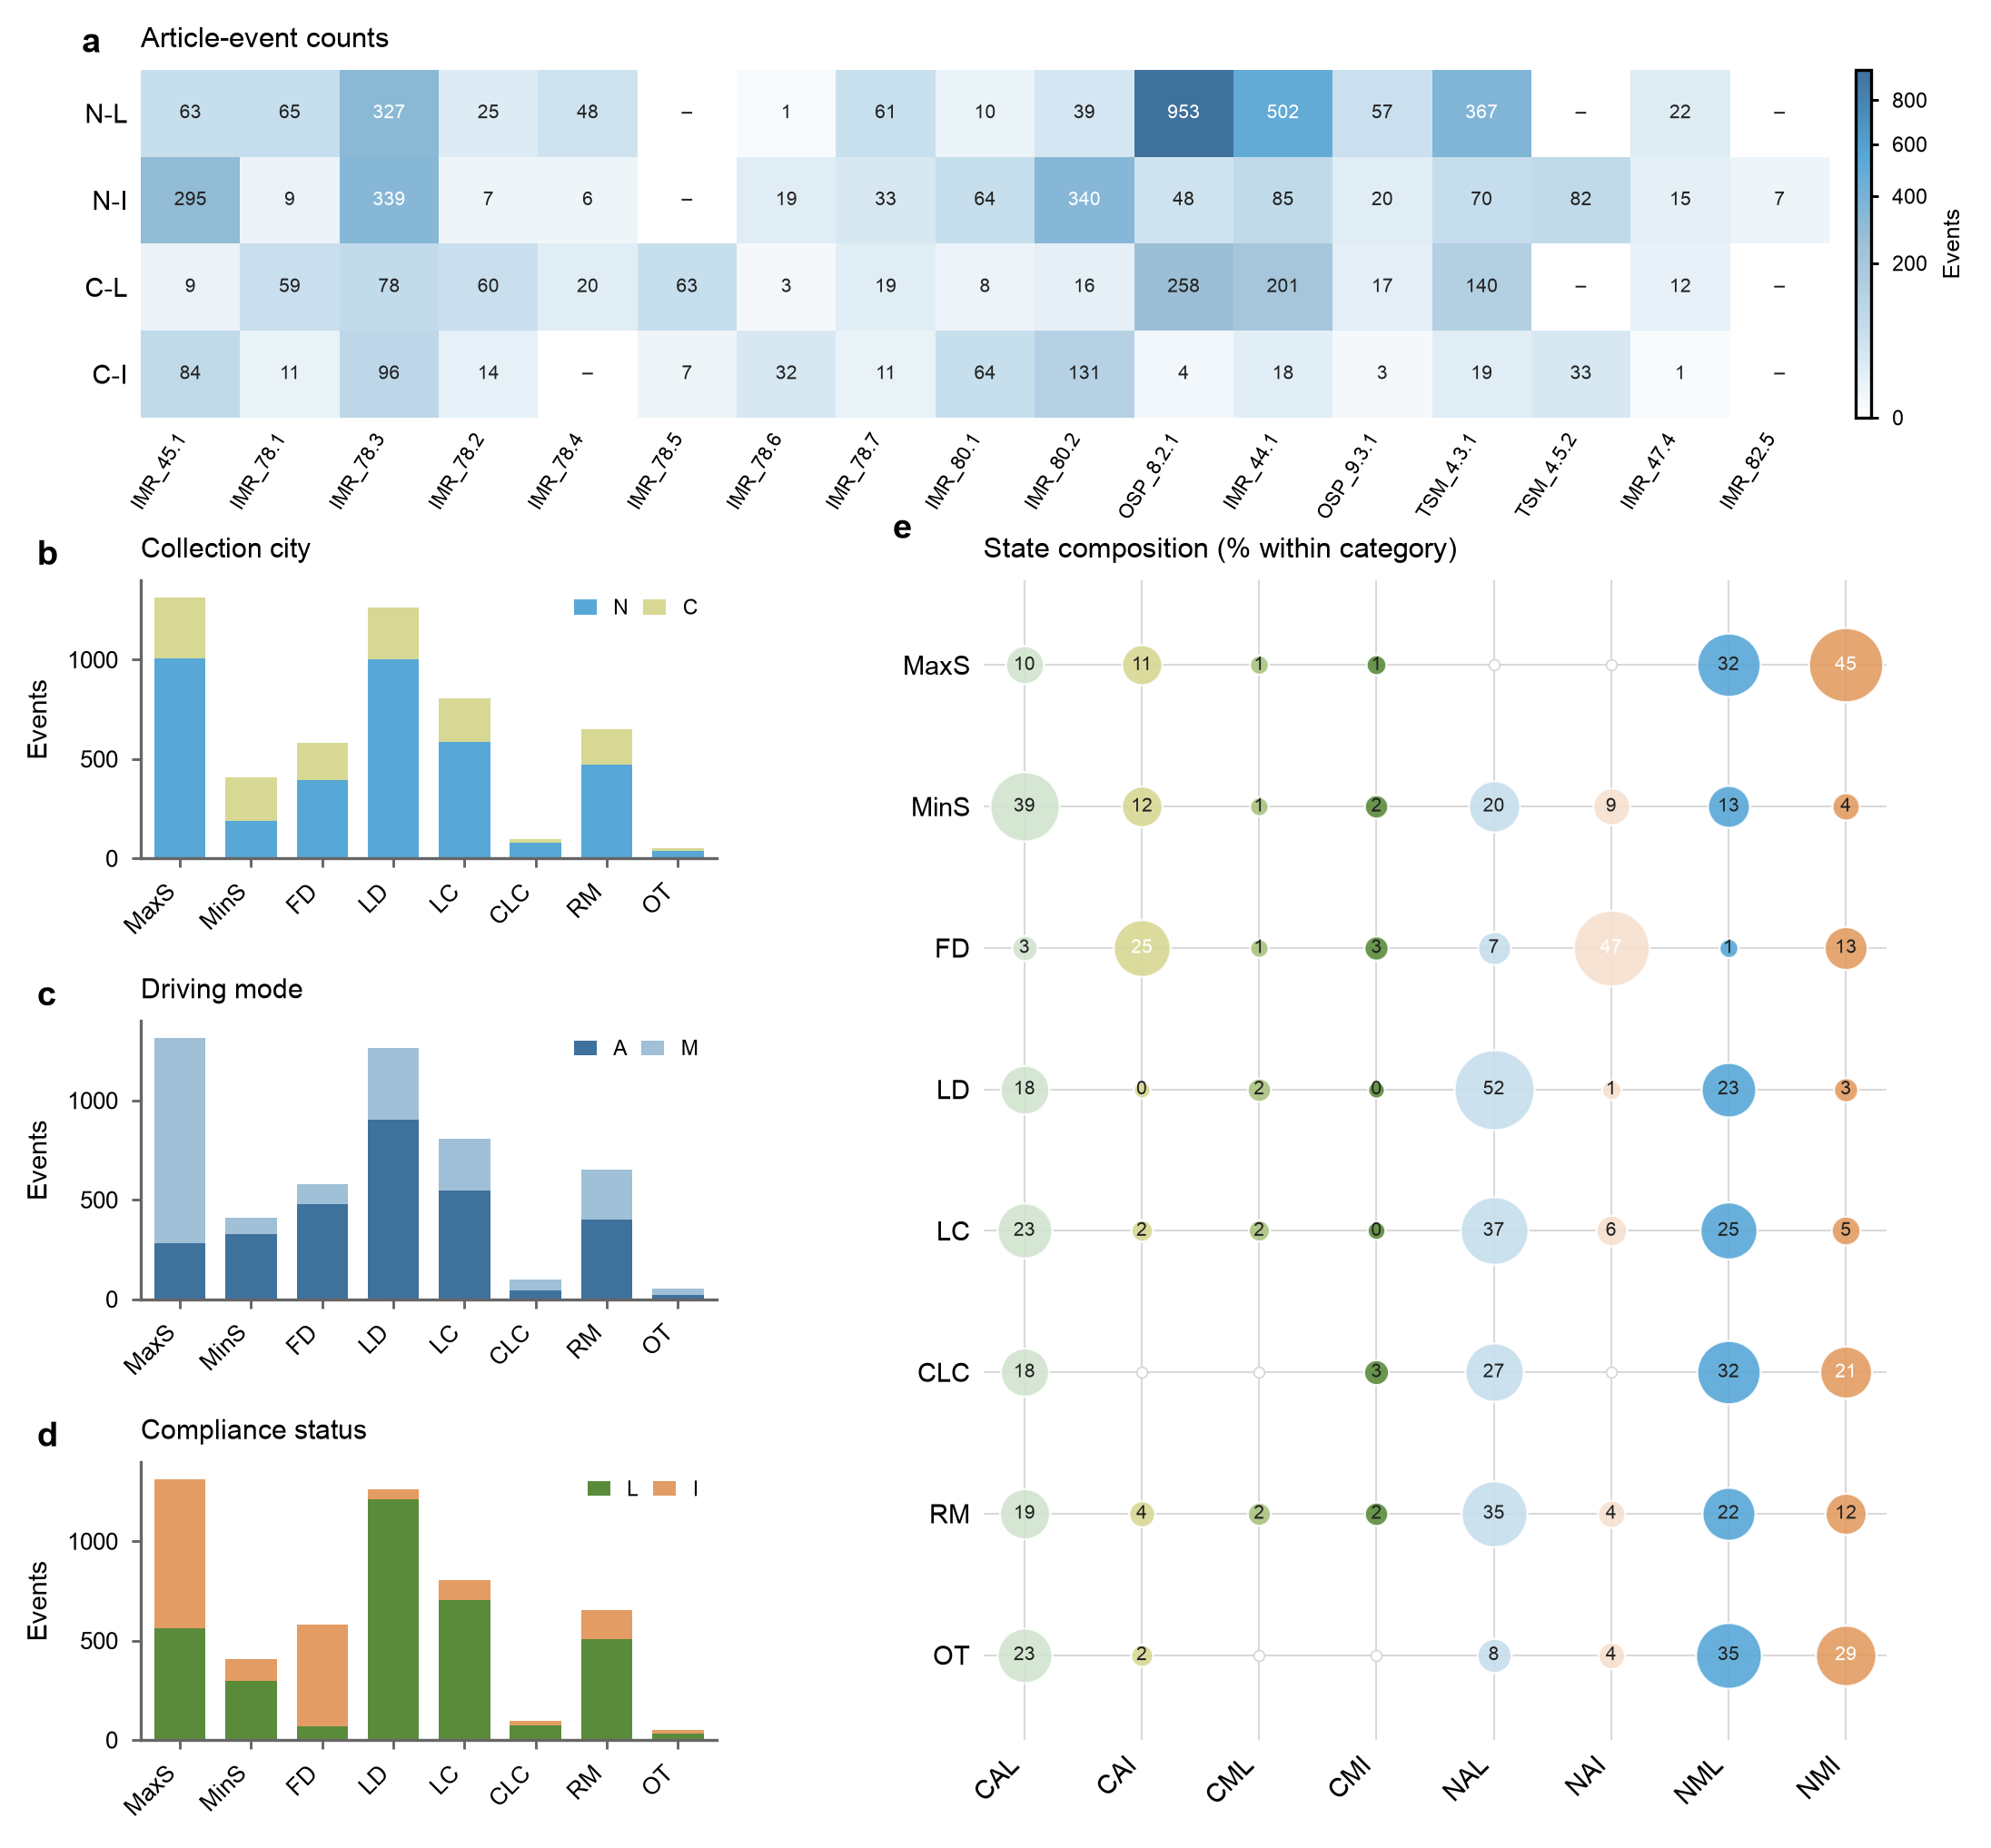
\includegraphics[width=0.96\textwidth]{fig5.png}
% TLCD 1.0 的事件级数据构成。(a) 按采集城市和合规状态分层的法规条款事件数；(b--d) 8 类事件按城市、驾驶模式和合规状态的数量；(e) 8 种联合状态在各事件类别内的百分比。
\caption{Event-level composition of TLCD 1.0. (\textbf{a}) Article-event counts stratified by collection city and compliance status. (\textbf{b--d}) Counts for the eight event categories stratified by collection city, driving mode and compliance status. (\textbf{e}) Within-category percentages for the eight joint states. N and C denote Nanjing and Changchun, A and M denote automated and manual driving, and L and I denote compliant and violation events, respectively. Category abbreviations are MaxS, maximum speed limit; MinS, minimum speed limit; FD, following distance; LD, lateral distance; LC, lane change; CLC, continuous lane change; RM, road marking; and OT, overtaking. Bubble area in (\textbf{e}) is proportional to the within-category percentage, with values shown inside the bubbles.}
\label{fig:event-statistics}
\end{figure*}

% 为表征数据集的场景多样性，图 6 同时展示了各事件类别内互斥的主场景子类，以及全部 5,173 个事件中可重叠的道路、设施和交通/环境属性。特殊场景标签呈现长尾分布，因此使用者在构建训练与测试子集时应保留实际的类别和场景频率。
Figure~\ref{fig:scenario-diversity} summarizes two complementary dimensions of scenario diversity: mutually exclusive primary subtypes within each event category and non-exclusive road, facility and traffic/environment attributes across all 5,173 events. The contextual labels followed a long-tailed distribution, which should be considered when defining training and evaluation subsets.

\begin{figure*}[htbp]
\centering
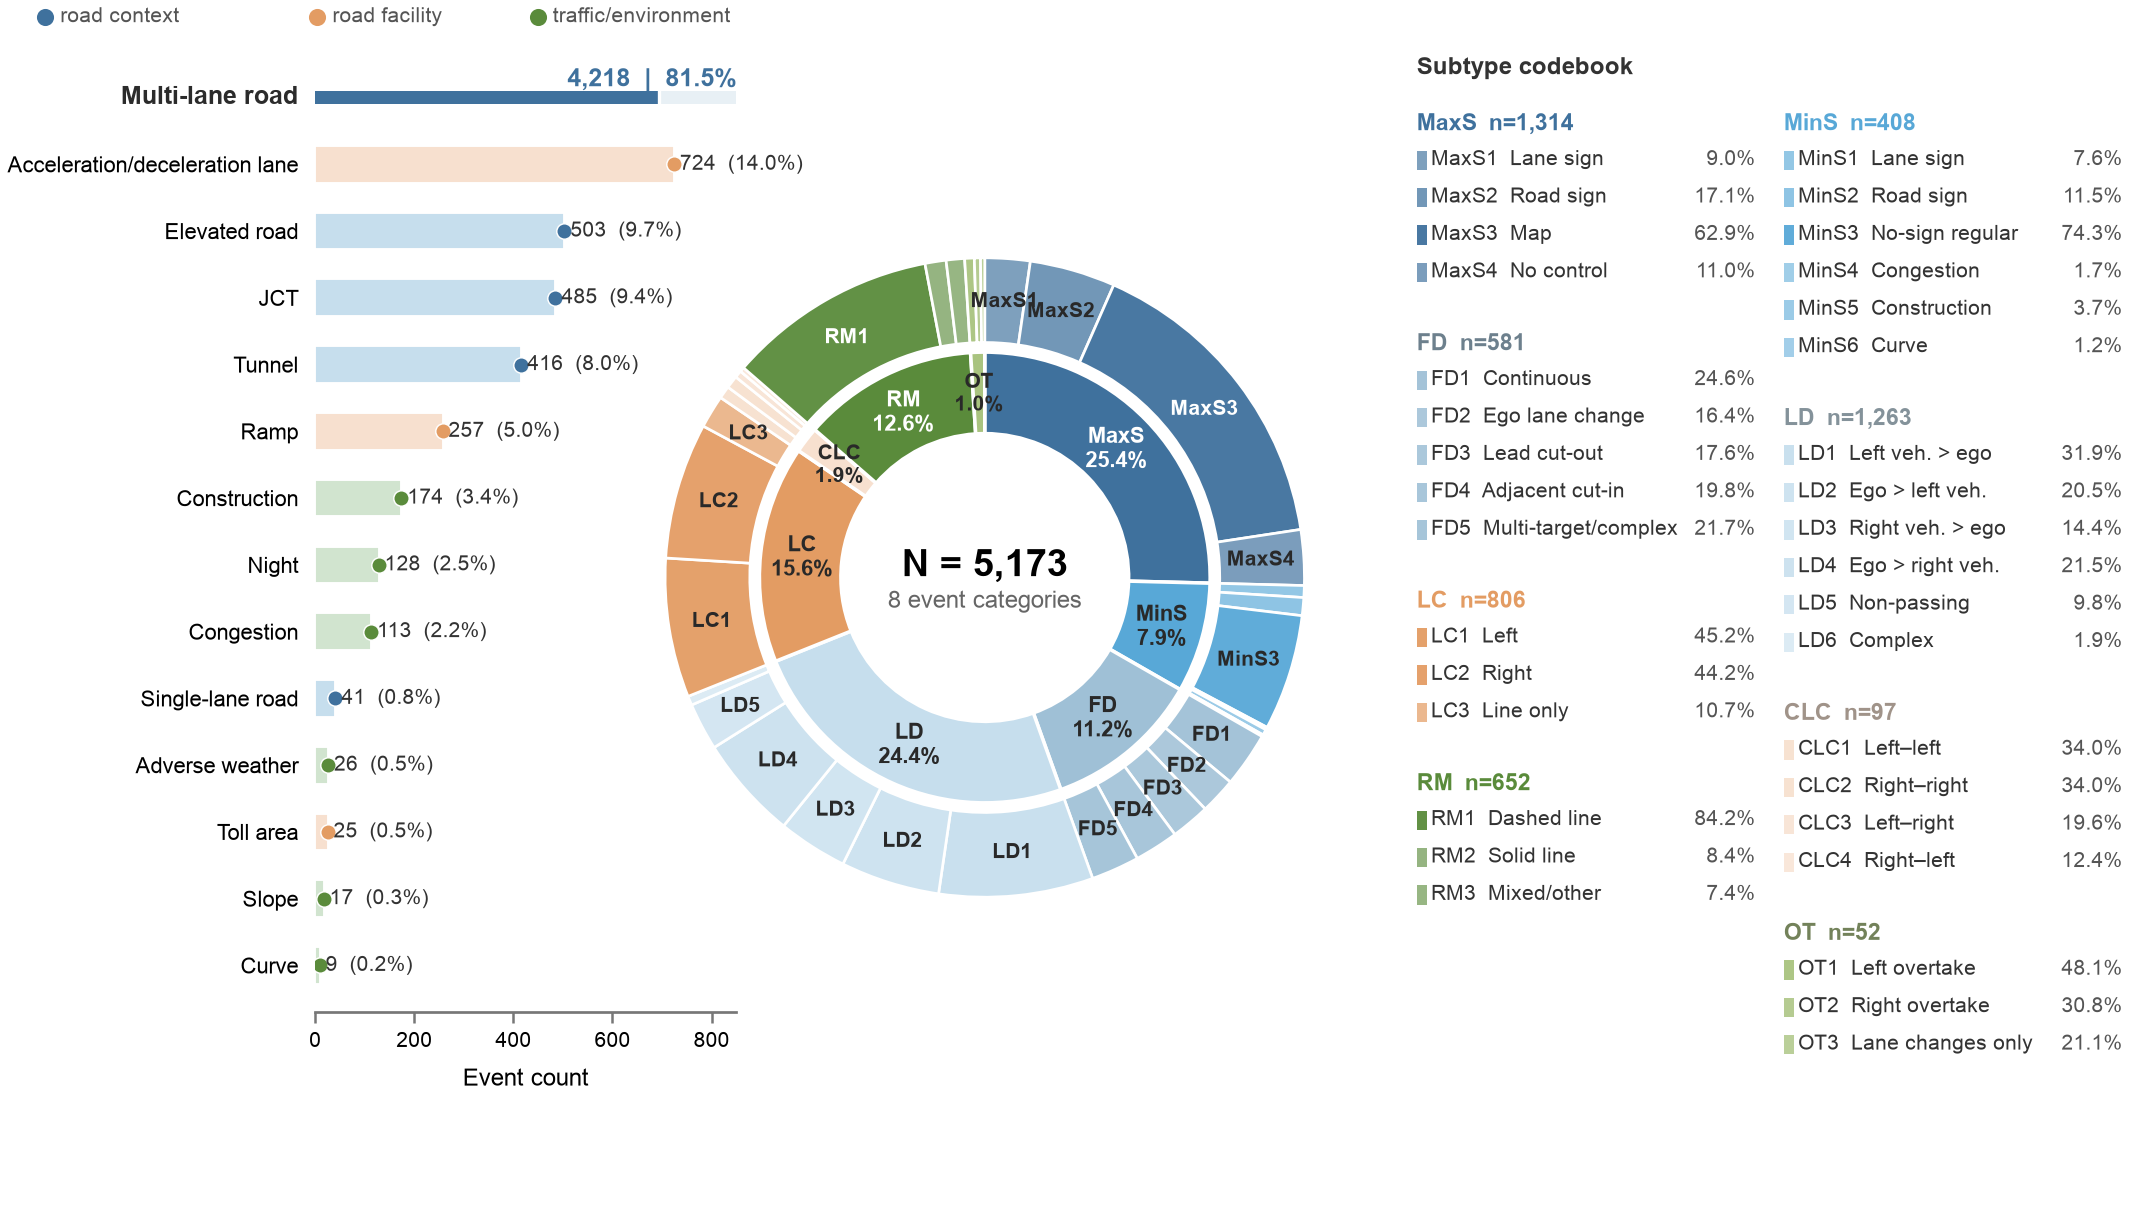
\includegraphics[width=0.98\textwidth]{fig6.png}
% TLCD 1.0 的事件子类和上下文场景多样性。双环图将 8 个事件类别（内环）与类别内互斥的主子类（外环）相联系；柱状图给出可重叠上下文标签的事件数及其占数据集的比例。
\caption{Event-subtype and contextual diversity of TLCD 1.0. The central double-ring chart links the eight event categories (inner ring) to mutually exclusive primary subtypes within each category (outer ring). Inner-ring percentages use all 5,173 events as the denominator; the subtype codebook reports percentages within the corresponding event category. The bar chart shows event counts and dataset-level percentages for non-exclusive contextual labels, coloured by road context, road facility and traffic/environment attributes. Because contextual labels are non-exclusive, their counts can sum to more than the dataset total.}
\label{fig:scenario-diversity}
\end{figure*}

\FloatBarrier

\section{Technical Validation}\label{sec:technical-validation}

% TODO：待完成并核对质量检查后填写。预计仅保留必要内容：
% 1. 事件目录、JSON/CSV 可读性和必需字段的完整性；
% 2. EgoInfo、ObjInfo、MapInfo 与 EvidenceChain 的 event_time 对齐；
% 3. 抽样视频复核和合规标签一致性；
% 4. 已知的缺失、异常与排除规则。
[To be drafted after completion of the technical quality checks.]

\section{Usage Notes}\label{sec:usage-notes}

% TODO：简要说明 CSV/JSON/视频的联合使用、类别不平衡、分组划分建议，以及 VLM 生成文本不参与合规标签确定的边界。
[To be drafted after the final repository package has been checked.]

\section{Data Availability}\label{sec:data-availability}

% TODO：填写正式数据仓库、DOI/持久标识符、版本号和数据引用。
[Repository name, persistent identifier, version and dataset citation to be added.]

\section{Code Availability}\label{sec:code-availability}

% TODO：说明事件整理、质量检查和统计代码的获取地址、版本和许可证。
[Code repository, archived release and software licence to be added.]

\section*{Acknowledgements}

% TODO：填写必要的致谢信息。
[To be completed.]

\section*{Author Contributions}

% TODO：按 CRediT 或期刊要求填写作者贡献。
[To be completed.]

\section*{Funding}

% TODO：填写资助机构和项目编号。
[To be completed.]

\section*{Competing Interests}

% TODO：由全体作者确认后填写。
The authors declare no competing interests.

\backmatter

% TODO：当前 ref.bib 仍包含模板参考文献，后续应在全稿定稿时清理未使用条目。
\bibliography{ref}

\end{document}
